%%%  Pacchetto di stile A4  %%%
\documentclass[12pt,a4paper,oneside,italian]{book}
\usepackage[italian]{babel} 
\usepackage[T1]{fontenc} 
\usepackage[utf8]{inputenc}
\usepackage{phdthesis} % Pacchetto di stile per le tesi
% Ridefiniamo la riga di testa delle pagine:
\usepackage{fancyhdr}
\pagestyle{fancy}
\usepackage{titlesec}
\usepackage{setspace}
\usepackage{wrapfig}
\usepackage{sectsty}
\usepackage{lipsum}
\usepackage[font=footnotesize]{caption}
\usepackage{listings} %Per inserire codice
\usepackage[usenames]{color} %Per permettere la colorazione dei caratteri 
\definecolor{dkgreen}{rgb}{0,0.6,0}
\definecolor{gray}{rgb}{0.5,0.5,0.5}
\definecolor{mauve}{rgb}{0.58,0,0.82}

\definecolor{lightgray}{rgb}{.9,.9,.9}
\definecolor{darkgray}{rgb}{.4,.4,.4}
\definecolor{purple}{rgb}{0.65, 0.12, 0.82}
\renewcommand{\chaptermark}[1]{\markboth{#1}{}}
\renewcommand{\sectionmark}[1]{\markright{\thesection\ #1}}
\fancyhf{}
\fancyhead[RO]{\thepage}
\fancyhead[LO]{\leftmark}
\renewcommand{\headrulewidth}{0.1pt}
\renewcommand{\footrulewidth}{0pt}
\headsep=20pt
\sectionfont{\Large} 
\subsectionfont{\itshape\large} 
\titleformat{\chapter}[display]
  {\normalfont\huge\bfseries}{\chaptertitlename\ \thechapter}{20pt}{\huge}
\titlespacing*{\chapter}{0pt}{-10pt}{40pt}

\setlength{\skip\footins}{1cm}
\setlength{\footnotesep}{0.4cm}

\graphicspath{{./images/}}	% path directory figure
\linespread{1.5}	% interlinea
%%%%%%

\usepackage{graphics,graphicx}

\usepackage{amsmath,amsfonts,amssymb,amsthm} % pacchetti tipici per scrivere matematica  
\usepackage{latexsym}
\usepackage{array}
\usepackage{tocbibind}

\usepackage{cite}
\usepackage{color}

\usepackage{textcomp}
\usepackage{caption}
\usepackage{subcaption}
% TOC INFO: sono le info salvate nelle proprieta' del file pdf
\hypersetup{ 
  pdftitle=Relazione Elementi Software Dependability,
  pdfauthor=Lorenzo Cioni Saverio Meucci Tommaso Mugnai,
  pdfsubject=Modellazione e verifica di un sistema distribuito di sollevamento con SCADE
}    

%%%  Frontespizio  %%%

\university{}	% Universita' degli Studi di xxx (Firenze)
\faculty{Scuola di Ingegneria} %Nome della Scuola
\degree{}
\dept{} % nome dipartimento
\course{Corso di Laurea Magistrale in Ingegneria Informatica} %Corso di Laurea

\accademicyear{Anno Accademico 2015/2016} %anno accademico
\supervisor{Prof. Enrico Vicario} % relatore
\author{Lorenzo Cioni, Saverio Meucci}

%titolo in italiano
\title{\textbf{Testing di microarchitetture Java con JUnit e Mockito}}


%%%  BEGIN DOCUMENT  %%%
\begin{document}

%%%  FRONT MATTER  %%%
\frontmatter
\maketitle  	% stampa la pagina di frontespizio

\tableofcontents

%% Corpo della tesi

\mainmatter{
\section{Introduzione}

\chapter{Microarchitetture}

Le micro-architetture discusse di seguito sono state ideate avendo come base i testi degli esami del corso di Ingegneria del Software nell'anno 2016. In particolare sono stati scelti tre esami fra i più adatti al tipo di elaborato in oggetto.
Tali esercizi sono stati poi modificati ed estesi, con funzionalità e nuove classi, per renderli più interessanti nelle fasi successi di analisi e testing.

\section{Termostato}

Il sistema considerato riguarda una gestione semplificata di apparecchiature di riscaldamento mediante l’uso di un termostato. 

Ciascun apparecchio si comporta in modo specifico in base allo stato in cui si trova, dipendente dalla relazione tra la temperatura da lui rilevata tramite un sensore e quella impostata dal termostato. 

Se la temperatura rilevata è inferiore a quella impostata, il sistema passa nello stato ON; se le due temperature sono equivalenti, passa nello stato READY; se la temperatura rilevata è maggiore di quella impostata passa nello stato OFF. 

In base allo stato viene poi eseguita una procedura specifica (preparazione, accensione, spegnimento).

Questa micro-architettura è stata implementata sulla base del testo di esame di Ingegneria del Software del 21 gennaio 2016, il cui testo è riportato di seguito.

\vspace{0.5cm}

\emph{Si considerino i design patterns Observer e Strategy, la cui struttura è richiamata qui di seguito:
}
\begin{figure}[h]
    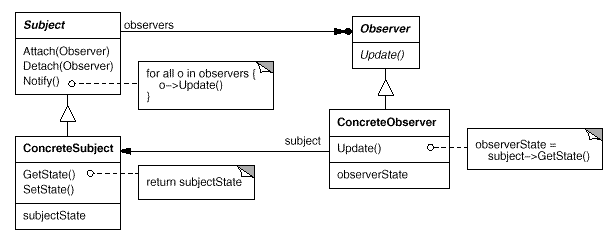
\includegraphics[scale=0.5]{../images/observer.jpg}
\end{figure}

\begin{figure}[h]
    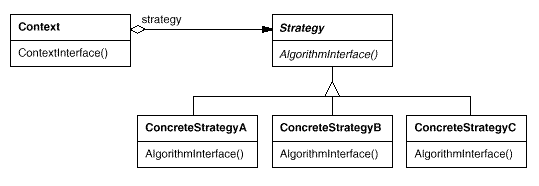
\includegraphics[scale=0.5]{../images/strategy.jpg}
\end{figure}

\emph{Si consideri uno scenario che combina i due patterns per realizzare un meccanismo di adattamento:
il Context è registrato come Observer su un qualche oggetto che opera come Monitor dell'ambiente di operazione; quando il Monitor rileva una variazione nello stato di operazione, il Context dello Strategy riceve notifica e adatta di conseguenza la Strategy con cui viene eseguita una qualche operazione.
Si descriva la struttura con cui vengono composti i due patterns, il Monitor e un Client che opera nel ruolo di test driver (il main) attraverso l'uso di un class diagram (8 punti)
Si illustri il funzionamento dello schema attraverso un sequence diagram riferito a uno scenario caratterizzante (6 punti);
Si dettaglino frammenti di codice della realizzazione che illustrano gli aspetti salienti dello schema, e si definisca uno scenario di test, realizzato per semplicità nella forma di un main(),  che esercita lo schema in no scenario che ne caratterizza l'intento (8 punti).}

\vspace{0.5cm}

Il sistema è implementato mediante l’utilizzo della combinazione di due design patterns, \emph{Observer} e \emph{Strategy}. Ciascun apparecchio rappresenta un \emph{Soggetto} che verrà monitorato da un \emph{Controller} (con la funzione di Observer). Al variare della temperatura rilevata dal \emph{Soggetto}, questa verrà notificata al suo \emph{Controllore} che andrà ad eseguire una strategia dipendente dallo stato in cui si trova il sistema.


\section{Copia difensiva}

La micro-architettura rappresenta un sistema di gestione degli esami da parte di uno studente. 

Ciascuno studente  ha un proprio libretto, in cui gli esami vengono inseriti. Il corso di laurea, utilizzando il libretto di uno studente, è in grado di calcolare la media dei voti degli esami. 

Sono previste funzionalità per il recupero e la modifica di un singolo esame, il recupero di tutti gli esami, l'aggiunta di un nuovo esame e la cancellazione di un singolo esame o di tutti gli esami presenti nel libretto di uno studente.

Questa micro-architettura è stata implementata sulla base del testo di esame di Ingegneria del Software del 17 giugno 2016, il cui testo è riportato di seguito.

\vspace{0.5cm}

\textit{Si illustri la pratica della copia difensiva nella seguente logica di dominio realizzata in Java:
}
\textit{La classe Studente ha un riferimento a un oggetto di tipo Libretto, il quale rappresenta la collezione degli Esami sostenuti dallo studente. Assumiamo che il riferimento al Libretto sia privato e che solo l'oggetto di tipo Studente che lo contiene lo possa modificare.}

\textit{La classe CorsoDiLaurea espone:
\begin{itemize}
\item un metodo getMedia(Libretto lib) che riceve il riferimento a un Libretto e calcola la media secondo le regole del particolare corso di laurea.
\end{itemize}}


\textit{La classe Studente espone:
\begin{itemize}
\item un metodo costruttore Studente(Libretto lib) che riceve come parametro un riferimento a un Libretto già inizializzato e che ha la responsabilità di creare l'oggetto di Studente componendo al suo interno l'oggetto di tipo Libretto;
\item un metodo pubblico getMedia(CorsoDiLaurea cdl) che riceve come parametro un riferimento a un oggetto di tipo CorsoDiLaurea e realizza il metodo per forwarding invocando il metodo getMedia sul corso di laurea.
\end{itemize}}


\textit{Si realizzi una descrizione UML della logica di domino (5 punti).
Si motivi la convenienza di realizzare una copia difensiva al momento della creazione di un oggetto di tipo Studente e al momento della invocazione del metodo getMedia sull'oggetto di tipo Studente (8 punti).}

\textit{Si riportino frammenti di codice che illustrano i tratti salienti dell'implementazione (10 punti.) }

\vspace{0.5cm}

Il sistema è implementato utilizzando la tecnica della \emph{copia difensiva}, ovvero invece di condividere l'oggetto originale, nel caso di studio il libretto o l'esame, viene condivisa una copia di esso, in modo da limitare gli effetti negativi di modifiche inattese.


\section{Generatore di espressioni booleane}

Il sistema considerato riguarda la creazione di espressioni booleane, potendo combinare fra di loro variabili booleane, operatori logici quali AND, OR, NOT e l'uso di parentesi.

Esso è in grado di valutare correttamente tali espressioni booleane e di stamparle a schermo, mostrando il valore assegnato alle singole variabili più la valutazione finale dell'intera espressione.

Questa micro-architettura è stata implementata sulla base del testo di esame di Ingegneria del Software del 26 febbraio 2016, il cui testo è riportato di seguito.

\vspace{0.5cm}

\textit{Si considerino i design patterns Composite e Builder.}

\begin{figure}[h]
    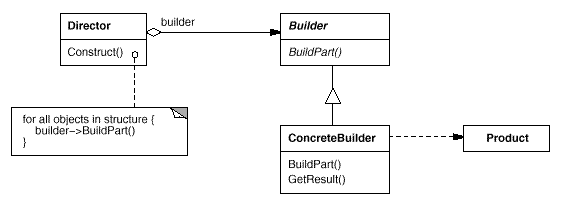
\includegraphics[scale=0.5]{../images/builder.jpg}
\end{figure}

\begin{figure}[h]
    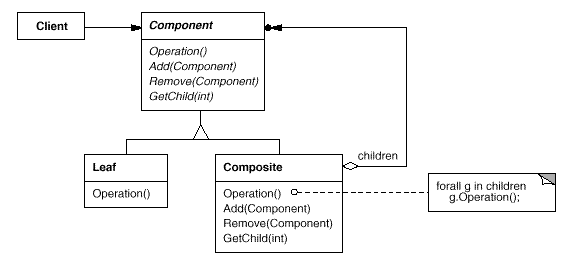
\includegraphics[scale=0.5]{../images/composite.jpg}
\end{figure}

\textit{Si consideri uno scenario che combina i due patterns per costruire e rappresentare
un'espressione Booleana:
\begin{itemize}
\item lo schema del Composite viene applicato per rappresentare e valutare un'espressione
Booleana nella quale un insieme di variabili possono essere combinate attraverso i
connettivi AND e OR e attraverso l'operatore di parentesi ().
[Suggerimento: le variabili sono rappresentate come istanze di Leaf, i connettivi AND,
OR e la parentesi ()sono rappresentati come istanze di subclassi di Composite.]
\item Lo schema del Builder viene applicato per costruire il Composite che rappresenta una
assegnata espressione.
[Suggerimento: il Builder espone i metodi per costruire una variabile, un AND, un OR
e una parentesi(); tali metodi restituiscono un riferimento a un Product, che nel caso
specifico è un Component; il Director tiene memoria dei Components messi in vita e li
usa per passarli al metodo di costruzione di ciascun Component]
\end{itemize}}


\textit{Si consideri in particolare lo scenario in cui il Builder mette in vita il Composite che
rappresenta l'espressione (X AND Y) Or Z, e in riferimento a questo caso:
\begin{itemize}
\item Si descriva la struttura con cui vengono composti i due patterns attraverso l'uso di un
class diagram (11 punti).
\item Si illustri il funzionamento dello schema attraverso un object diagram che
rappresenta gli oggetti messi in vita nella rappresentazione dell'espressione e quelli
usati per metterli in vita (8 punti);
\item Si dettaglino frammenti di codice della realizzazione che illustrano aspetti salienti
dello schema, e si definisca uno scenario di test, realizzato per semplicità nella forma
di un main(), che esercita lo schema in uno scenario che ne caratterizza l'intento (11
punti).
\end{itemize}}

\vspace{0.5cm}

Il sistema è implementato combinando i design patterns \emph{Composite} e \emph{Builder}. Il design pattern \emph{Composite} definisce le interfacce per creare le componenti semplici, le variabili, e le componenti composte, gli operatori e le parentesi. Il design pattern \emph{Builder} si occupa di istanziare correttamente tali componenti e di combinarle fra di loro per creare delle espressioni booleane più complesse.

\section{\emph{Fault models}}

Un \emph{fault model}, nell'ambito software, è un modello che rappresenta ciò che può andare storto durante l'operazione di un programma. Grazie a questo modello, è possibile predire le conseguenze dei vari faults.

Nel nostro caso, i faults individuati sono sia legati alla struttura stessa del sistema, dipendente dai design pattern utilizzati per realizzare le micro-architetture, sia legati al tipo di problema specifico, come ad esempio vincoli su certi valori.

\subsection{Termostato}

In questa micro-architettura, le criticità sono principalmente legate ai design patterns utilizzati, nello specifico i design patterns \emph{Observer} e \emph{Strategy}.

I possibili faults dell'\emph{Observer} riguardano innanzitutto la registrazione e la rimozione di observer da parte di un device, ovvero del soggetto osservato. In particolare, può avvenire una registrazione non corretta quando viene instanziato un observer ma non viene registrato dal Device, ovvero non è inserito nella sua lista di observers da notificare; la criticità della rimozione di un observer è legata al caso in cui, distrutto l'oggetto observer, questo rimane referenziato dal qualche parte, ad esempio nella lista degli observer di un device. Tale situazione può portare al caso in cui qualcuno nell'esecuzione del programma possa chiedere a quell'observer, distrutto, di fare qualcosa.
Infine, per quando riguarda tale design pattern, un possibile fault è legato alla fase di aggiornamento della temperatura nei singoli devices (soggetti) nel caso in cui non vengano notificati tutti gli observers a lui associati.

Per quanto riguarda invece il design pattern \emph{Strategy}, la criticità è legata ad una non corretta esecuzione della giusta strategia, dipendente dalla temperatura rilevata, al cambio di stato del device.


\subsection{Copia difensiva}

Questa micro-architettura non fa utilizzo di design patterns ma implementa la tecnica della \emph{copia difensiva}. Il fault legato a tale strategia riguarda un'errata copia dell'oggetto, ovvero se non tutti i suoi attributi sono copiati correttamente. Ciò può portare ad utilizzare attributi che nell'oggetto originati sono instanziati, ma nella copia non lo sono, cosicché il programma tenta di usare \emph{null} quando invece è richiesto un oggetto.

Il fault legato alla copia difensiva può manifestarsi durante l'inserimento di un esame in un libretto, poichè viene inserita una copia dell'oggetto Esame, così come durante il calcolo della media dei voti degli esami presenti in un libretto, poichè ciò che viene passato all'oggetto di classe DegreeCourse è una copia dell'oggetto Transcript (libretto).

Altre possibili criticità, legate al tipo di problema specifico, riguardano l'assegnamento dei voti agli esami e il calcolo della media.
Per quanto concerne l'assegnamento dei voti agli esami, esso deve rispettare dei vincoli di range dei valori, in questo caso fra 18 e 30 compresi, ed altrimenti generare un'eccezione e ritenere quindi l'assegnamento del voto non valido cosiccè l'esame non aggiorni il suo attributo legato al voto.
Il fault legato ad un calcolo errato della media dei voti degli esami può riguardare sia un'errata computazione sia all'impiego nel calcolo di esami ai quali è sono stato assegnato un voto, o all'impiego di esami che dovrebbero essere stati rimossi dal libretto considerato.

L'ultimo caso può verificarsi se, per qualche motivo, la rimozione degli esami viene fatto su un libretto copia diverso da quello che viene passato al corso di laura per fare il calcolo della media.


\subsection{Generatore di espressioni booleane}

Questa micro-architettura implementa un generatore di espressioni booleani tramite l'utilizzo dei design patterns \emph{Builder} e \emph{Composite}.

Le criticità legate al \emph{Composite} riguardano in particolare il metodo \textit{add} che permette di aggiungere componenti ad altri componenti. I componenti leaf non possono tuttavia eseguire tale operazione a differenza dei componenti composite. L'implementazione base del metodo \emph{add} è realizzata nella classe astratta Component, assumento come caso base quello di componenti leaf e generando così un'eccezione. L'implementazione del metodo \emph{add} per i componenti composite è lasciato alla classe Composite ed eventualmente alle classi che la estendono, tramite override.

I faults riguardanti il design pattern \emph{Builder} sono tutti quelli legati ad una costruzione di oggetti, in questo caso componenti e espressioni booleani, diversa da quella desiderata dal client che da solo delle istruzioni su come realizzare tali oggetti ma l'implementazione è affidata interamente all'oggetto Builder.

Infine, una criticità può essere legata nella fase di valutazione delle espressioni booleani e dei suoi componenti.
\chapter{Astrazione dei modelli}

Dato un \emph{fault model}, si procede con l'astrazione dei modelli mediante una qualche rappresentazione strutturale degli stessi.

Nel caso in esame, l'astrazione realizzata è il \emph{diagramma delle classi}, una rappresentazione che pone l'accento sulla struttura degli oggetti del sistema (classi di appartenenza, relazioni, attributi e operazioni).

Vengono qua riportati i diagrammi delle classi delle tre architetture in esame.

\begin{figure}[h] 
  \centering
    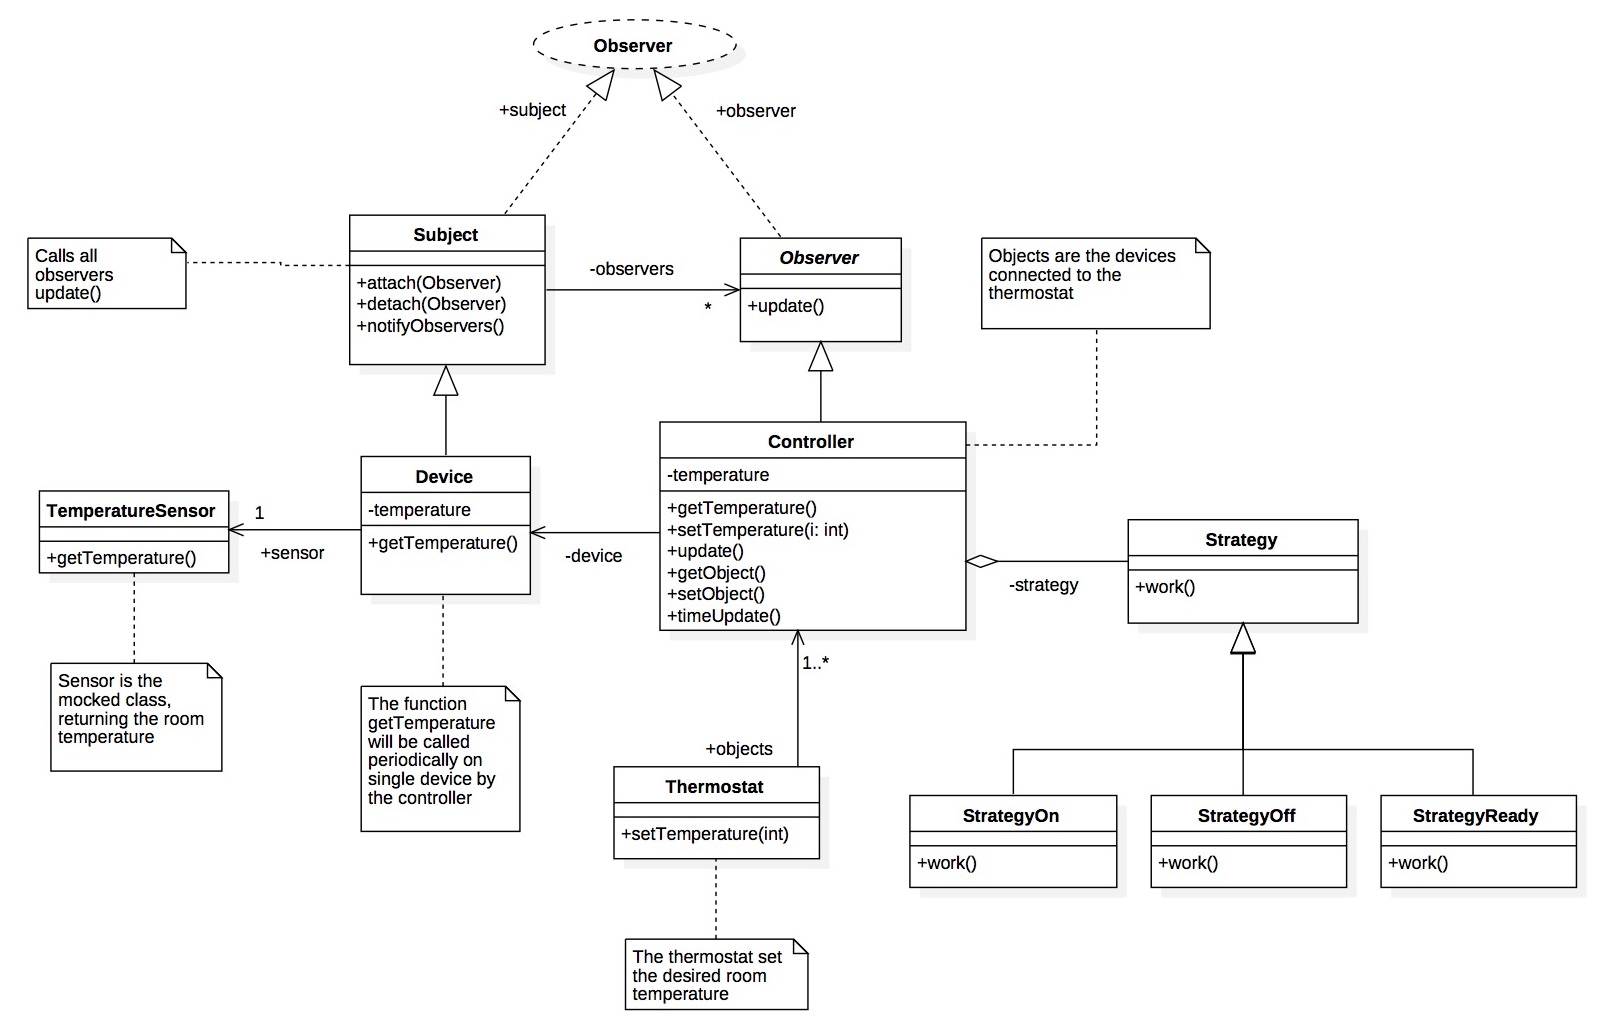
\includegraphics[width=1\textwidth]{ObserverStrategy.jpg}
    \caption{{\small \textit{Diagramma delle classi dell'architettura contenente l'Observer e lo Strategy, il Termostato}}}
\end{figure}

\begin{figure}[h] 
  \centering
    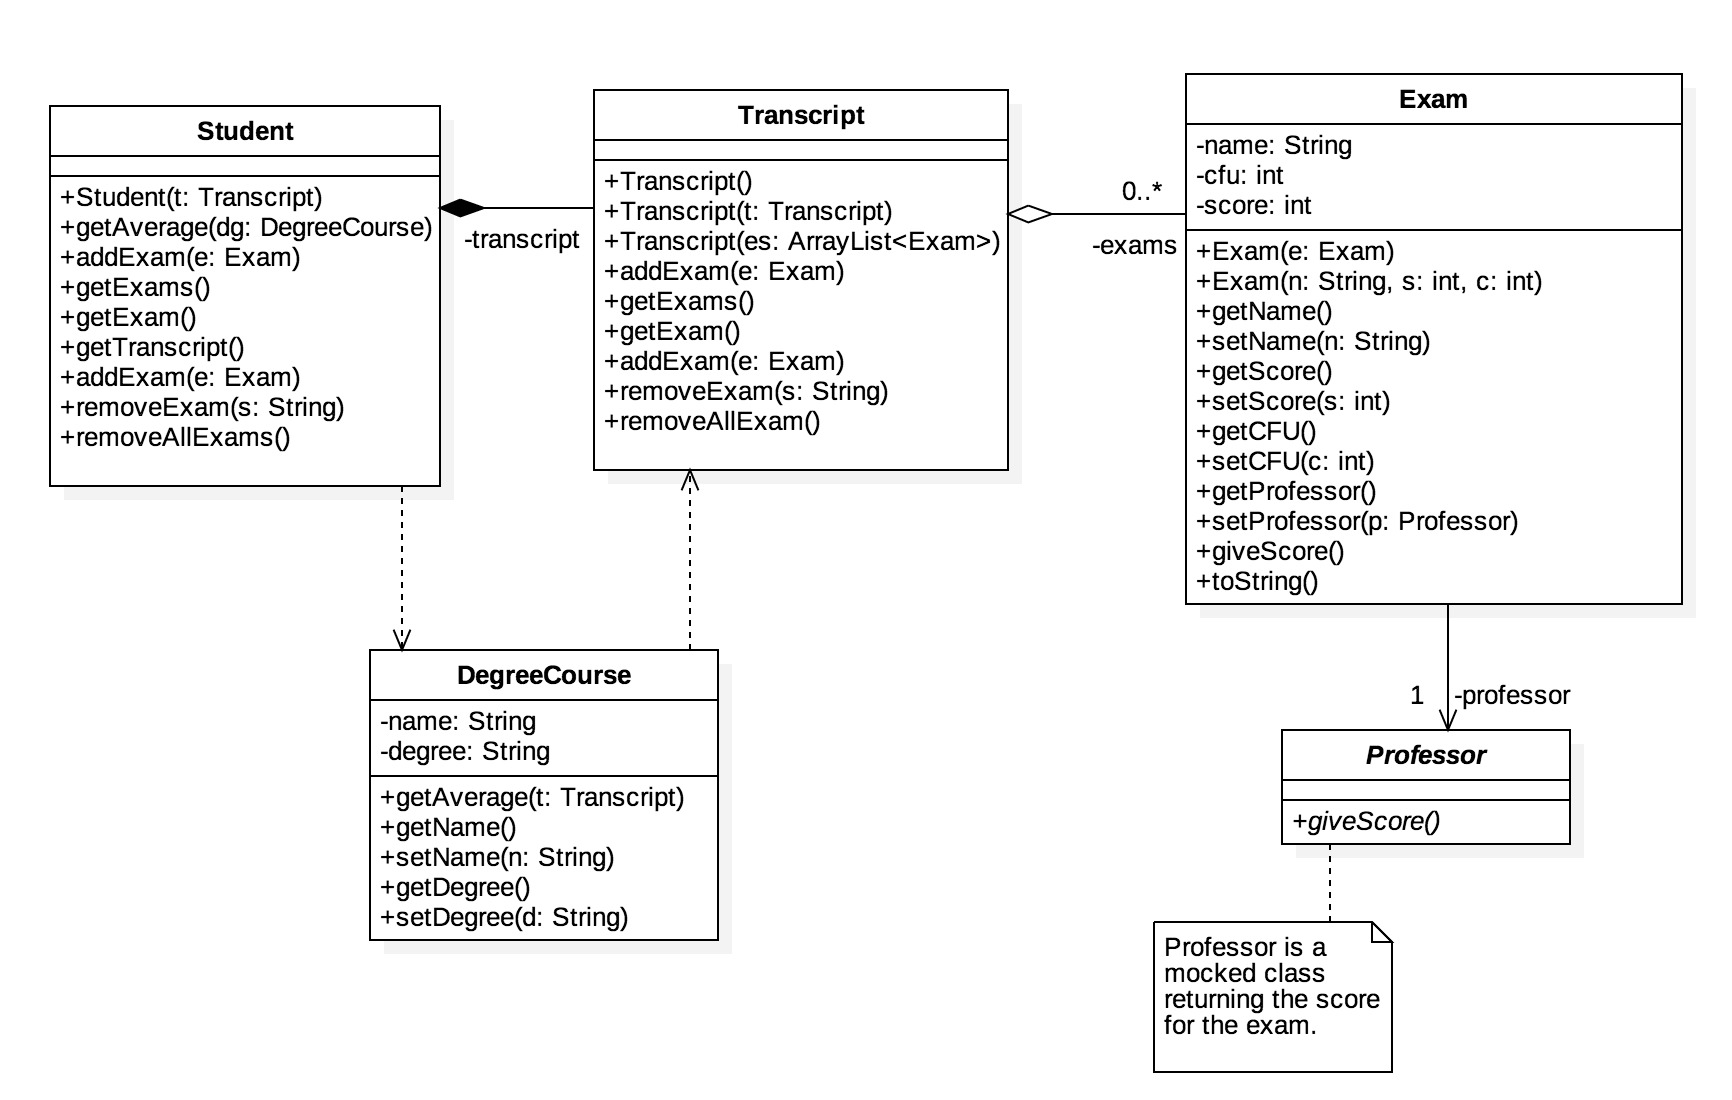
\includegraphics[width=1\textwidth]{defensivecopy.jpg}
    \caption{{\small \textit{Diagramma delle classi dell'architettura del sistema esami (copia difensiva)}}}
\end{figure}

\begin{figure}[h] 
  \centering
    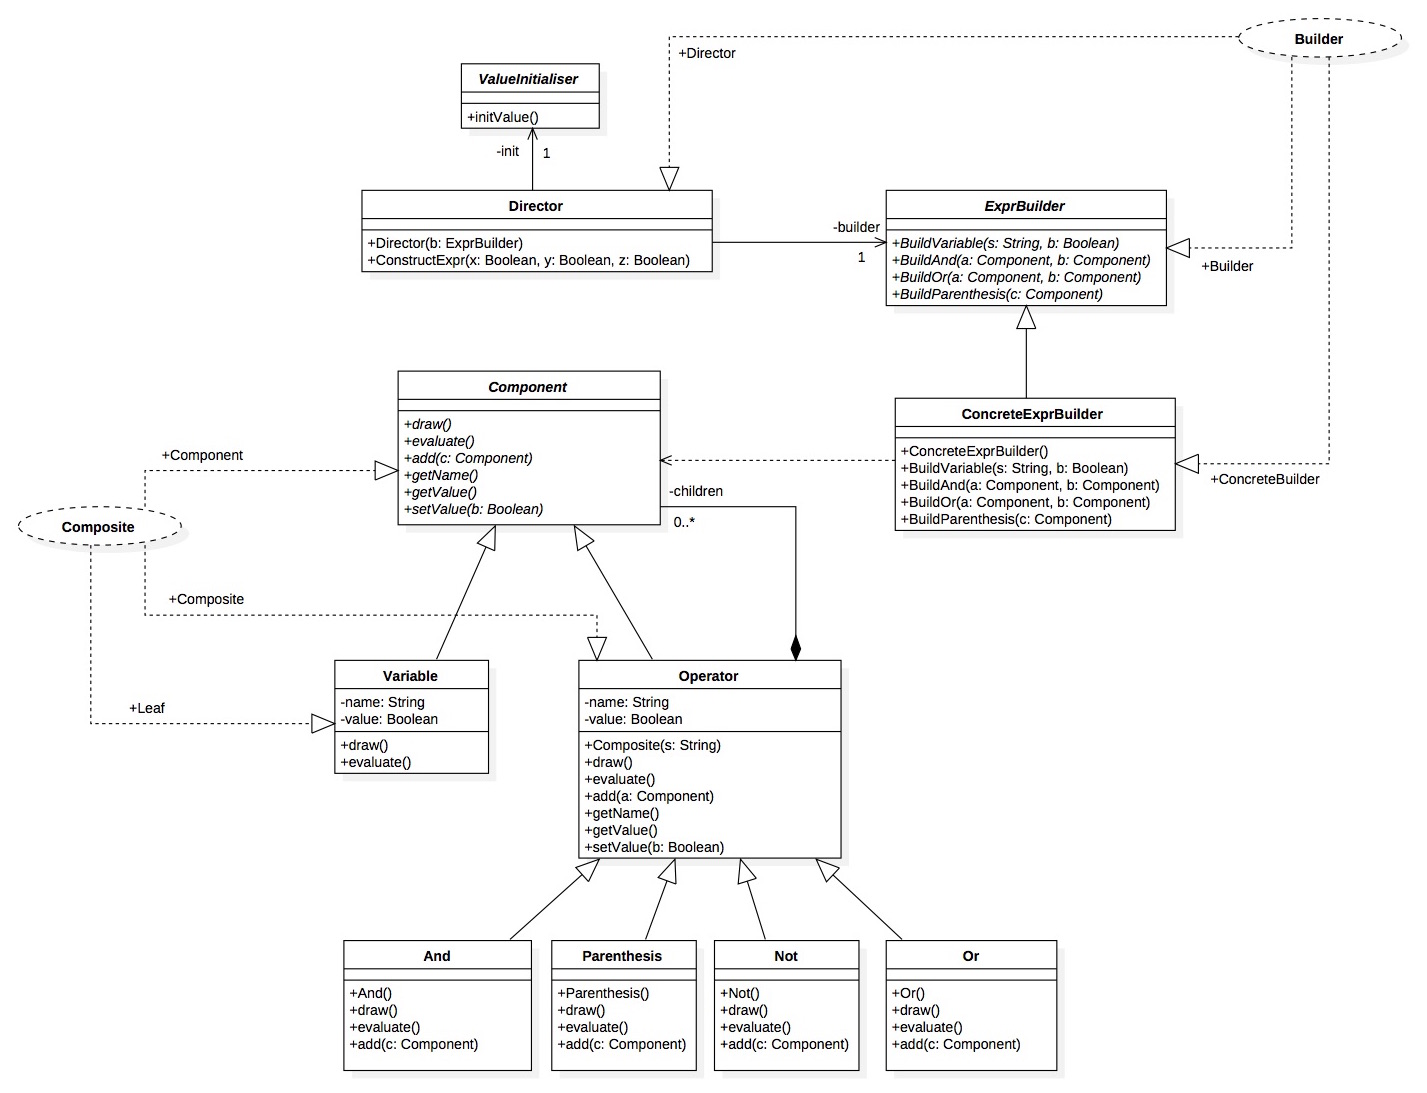
\includegraphics[width=1\textwidth]{buildercomposite.jpg}
    \caption{{\small \textit{Diagramma delle classi dell'architettura contenente il Builder ed il Composite, il generatore di espressioni booleane}}}
\end{figure}

Nel diagramma delle classi vengono inoltre evidenziati i \emph{design patterns} utilizzati mediante una serie di annotazioni dedicate. In questo modo è possibile focalizzare l'attenzione sulle criticità presenti nel \emph{fault model } e da questi dipendenti.

Grazie all'astrazione del modello così rappresentata, è possibile proseguire andando a definire un criterio di copertura adeguato a verificare le criticità esposte nel \emph{fault model}.

 %diagramma delle classi UML
\section{Criterio di copertura}

Il \emph{criterio di copertura} scelto per le architetture in esame è il \emph{functionality coverage}.

Il \emph{functionality coverage}, \emph{copertura di funzionalità}, indica che i test devono andare a verificare tutte le proprietà e le funzionalità previste nei requisiti.

Un altro criterio di copertura preso in considerazione era il \emph{function coverage} che prevede di andare a definire test in cui tutte le funzioni definite nel sistema siano state chiamate almeno una volta. In architetture così limitate però ciò si riduceva a un tipo di copertura, la \emph{statement coverage}, ancora più stringente, in cui i test devono verificare ciascuna linea di codice almeno una volta. 

Molto più interessante, nei casi presi in esame, era definire test che verificassero le già limitate funzionalità del sistema.
\section{Testing}

Una volta individuato il criterio di copertura ottimale, si procede con la definizione di una \emph{test suite}, un insieme di test che, se verificati, rispettano le specifiche imposte dal criterio scelto.

\subsection{Definizione della \emph{test suite}}

Per la creazione e la definizione della \emph{test suite} è stato utile rappresentare i possibili test in una tabella. Nella tabella è presente il numero del test (un progressivo identificativo del singolo test), il titolo (cosa riguarda il test), una descrizione (in cui viene esplicitato il risultato atteso del test) ed un indicatore per la sua corretta esecuzione o meno.

I test definiti verificano le funzionalità principali dei sistemi in esame, andando a coprire nella loro interezza le criticità esposte nel \emph{fault model}.

\begin{table}[h!]
\caption{Test suite - Termostato}
\centering % used for centering table
\begin{tabular}{|p{1cm}|p{3cm}|p{7cm}|p{1cm}|} % centered columns (4 columns)
\hline\hline %inserts double horizontal lines
\textbf{Num} & \textbf{Titolo} & \textbf{Descrizione} & \textbf{Stato} \\ [0.5ex] % inserts table
%heading
\hline % inserts single horizontal line
1 & Verifica stato iniziale & Inizialmente lo stato del soggetto osservato deve essere impostato su READY & OK \\ \hline% inserting body of the table
2 & Verifica aggiornamento della temperatura & Il termostato si comporta in modo differente in base alla temperatura rilevata dal componente, aggiornando lo stato del controllore e attuando la corretta strategia. Se la temperatura rilevata è minore a quella impostata dal termostato, lo stato del controllore è impostato a ON; se sono uguali è impostato a READY; altrimenti a OFF. & OK \\ \hline
3 & Verifica \emph{observers} iniziali & Inizialmente il numero degli \emph{observers} associati ad un soggetto è 0. & OK \\ \hline
4 & Aggiunta \emph{observer} & Quando un nuovo \emph{observer} è associato ad un soggetto, il numero degli \emph{observers} nella lista del soggetto aumenta correttamente di 1. & OK \\ \hline
5 & Rimozione \emph{observer} & Quando un \emph{observer} è rimosso da un soggetto, il numero di elementi nella sua lista diminuisce di 1. & OK \\ \hline
6 & Notifica agli \emph{observers} & Quando la temperatura rilevata dal dispositivo si aggiorna (cambia), tutti gli \emph{observers} presenti nella lista del dispositivo vengono notificati. & OK \\ [1ex] % [1ex] adds vertical space
\hline %inserts single line
\end{tabular}
\label{table:observerstrategy} 
\end{table}

\begin{table}[h!]
\caption{Test suite - Gestione libretto universitario}
\centering % used for centering table
\begin{tabular}{|p{1cm}|p{3cm}|p{7cm}|p{1cm}|} % centered columns (4 columns)
\hline\hline %inserts double horizontal lines
\textbf{Num} & \textbf{Titolo} & \textbf{Descrizione} & \textbf{Stato} \\ [0.5ex] % inserts table
%heading
\hline % inserts single horizontal line
1 & Creazione di un esame & Un esame è creato correttamente con il nome desiderato, i CFU impostati ed il voto impostato a -1 (valore di default) & OK \\ \hline% inserting body of the table
2 & Inserimento di un esame nel libretto & Un esame è correttamente inserito nel libretto. L'inserimento è effettuato mediante una copia difensiva dell'oggetto di tipo Esame. La lista degli esami contenuti nel libretto deve dunque aumentare di uno. & OK \\ \hline
3 & Associazione Studente-Libretto &Un libretto può essere associato ad uno studente. L'associazione è effettuata usando una copia difensiva dell'oggetto Libretto. & OK \\ \hline
4 & Assegnazione di un voto ammesso & Un professore può associare un voto ad un esame. Quando il professore imposta il voto a un esame, se questo si trova nel range tra 18 e 30, il valore del voto associato all'esame deve cambiare in accordo all'assegnamento. Il professore è una classe \emph{mocked}. & OK \\ \hline
5 & Assegnazione di un voto non ammesso & Quando un professore imposta un voto fuori dal \emph{range} prefissato (da 18 a 30) ad un esame, deve essere lanciata un'eccezione.  & OK \\ \hline
6 & Calcolo della media & Quando è richiesto il calcolo della media dei voti degli esami di uno studente, una copia del libretto è usata all'oggetto Corso di Laurea, effettuando dunque una copia difensiva. Tutti gli esami con un voto diverso da -1 (il valore di default) devono essere considerati nel calcolo della media. Verificare che la media calcolata automaticamente sia corretta. & OK \\ \hline
7 & Rimozione di un esame & Un esame può essere rimosso da un libretto. Da quel momento non deve più essere conteggiato nel calcolo della media dei voti. & OK \\ \hline
8 & Ripristino del libretto & Effettuando un ripristino del libretto tutti gli esami al suo interno sono correttamente rimossi. & OK \\ [1ex] % [1ex] adds vertical space
\hline %inserts single line
\end{tabular}
\label{table:defensivecopy}
\end{table}


\begin{table}[h!]
\caption{Test suite - Generatore espressioni booleane}
\centering % used for centering table
\begin{tabular}{|p{1cm}|p{3cm}|p{7cm}|p{1cm}|} % centered columns (4 columns)
\hline\hline %inserts double horizontal lines
\textbf{Num} & \textbf{Titolo} & \textbf{Descrizione} & \textbf{Stato} \\ [0.5ex] % inserts table
%heading
\hline % inserts single horizontal line
1 & Aggiunta di un componente ad una Variabile & La classe Variabile estende la classe astratta Componente. Quando il metodo \emph{add()} viene invocato su un'istanza della classe Variabile deve essere lanciata un'eccezione. & OK \\ \hline% inserting body of the table
2 & Aggiunta di un componente ad un operatore & La classe Operatore estende la classe astratta Component. Quando il metodo \emph{add()} viene invocato su un'istanza di una classe che estende la classe Operator, i componenti passati come parametri devono essere aggiunti alla lista dei componenti dei figli (senza lanciare alcuna eccezione). & OK \\ \hline
3 & Generatore di espressioni concrete & Quando un'espressione (Variable, And, Or, Not, Parenthesis) è costruita, deve avere gli attributi impostati nel modo corretto. & OK \\ \hline
4 & Valutazione e output di un'espressione & Una generica espressione booleana deve essere correttamente valutata per tutti i possibili valori delle variabili in essa contenute. L'output dell'espressione deve essere inoltre quello atteso, in accordo con la valutazione. I valori delle variabili sono inizializzati grazie ad una classe \emph{mocked} (ValuesInitialiser) ed il suo metodo \emph{initVar()}. & OK \\ [1ex] % [1ex] adds vertical space
\hline %inserts single line
\end{tabular}
\label{table:observerstrategy} 
\end{table}


\subsection{JUnit}

Per l'implementazione dei test definiti nella \emph{Test Suite} è stata utilizzata un framework Java per il testing di unità: JUnit\footnote{JUnit, versione 4 - http://junit.org/junit4/}.

Il \emph{test di unità} prevede di andare a verificare e testare le singole entità del mio sistema (classi o metodi) al fine si assicurarsi che le singole unità di sviluppo assolvano le funzioni seguendo i requisiti, facendo sì, in questo modo, che, integrandole in sistemi più complessi, continuino a rispettarli. 
L'idea alla base è dunque quella di valutare ogni singolo metodo (o funzionalità) del sistema in funzione dei valori attesi.

Il framework mette a disposizione degli sviluppatori un insieme di \emph{annotazioni Java}, volte a indicare i vari test da eseguire e quali operazioni compiere prima e dopo il test eseguito.

\begin{lstlisting}
import static org.junit.Assert.*;
public class ThermostatTest {
	...		
	@Before
	public void setup() {
		Strategy strategy = StrategyReady.getInstance();
		device = new Device();
		device.setSensor(sensor);
		controller = new Controller(strategy, device);	
		thermostat = new Thermostat();
		thermostat.addObject(controller);
		//Initialize thermostat to 20 degrees
		thermostat.setTemperature(20);
	}
\end{lstlisting}

Nell'esempio riportato sopra si nota la presenza di un metodo di inizializzazione (\emph{setup()}) che, grazie all'annotazione \emph{@Before} viene eseguito prima dell'esecuzione di ciascuna funzione test. Questo per consentire l'inizializzazione di variabili o attributi di classe utili per l'esecuzione del test stesso.

I metodi test (annotati opportunamente dall'annotazione \emph{@Test}) verranno eseguiti senza un ordine preciso, quindi non necessariamente vengono eseguiti nell'ordine definito. Un test fallisce se fallisce almeno uno dei metodi \emph{assert} contenuti in esso. I metodi assert sono metodi statici contenuti che effettuano una semplice comparazione tra il risultato atteso ed il risultato dell'esecuzione. 

\begin{lstlisting}
	/*
	 * Number: 1
	 * Title: Exam creation
	 * Description: An exam is created with the desired name, the desired 
	 * CFU and a default score of -1.
	 */
	@Test
	public void ExamCreationTest() {
		Exam exam = new Exam("Test Exam", 9);
		assertEquals("Exam name not correctly assigned.", "Test Exam", 
							exam.getName());
		assertEquals("Exam cfu not correctly assigned.", 9, exam.getCFU());
		assertEquals("Exam score not correctly initialised.", -1, 
							exam.getScore());	
	}
\end{lstlisting}

Nel caso precedente, che implementa il test numero 1 sul sistema della copia difensiva, viene verificato che un esame sia creato correttamente. Se una delle asserzioni fallisce, il test fallisce e vengono mostrati i messaggi specificati.

Un test anche potrebbe sollevare una eccezione: in questi casi è interessante l'uso del parametro \emph{expected} nell'annotazione dove diciamo che è attesa l'eccezione. Se il metodo non solleva quel tipo di eccezione il test sarà fallito.

\begin{lstlisting}
	/*
	 * Number: 1
	 * Title: Adding a component to a Variable.
	 * Description: Variable extends the abstract class Component. 
	 * When the add method of the Variable class 
	 * is called, an exception should be thrown.
	 * 
	 */
	@Test(expected=InvalidComponentAddingException.class)
	public void AddingComponentToVariableTest() throws 
								InvalidComponentAddingException {		
		ExprBuilder builder = new ConcreteExprBuilder();
		Component varx = builder.BuildVariable("X", true);
		Component vary = builder.BuildVariable("Y", false);
		varx.add(vary);
	}
\end{lstlisting}

Nel caso considerato è il test numero 1 sul sistema di generazione di espressioni booleane. Nel caso in cui il metodo \emph{add()} venga invocato su un'istanza della classe \emph{Variable} deve essere lanciata un'eccezione. Il test dunque è considerato passato se questa viene lanciata. 

Ciascun test presente nella Test Suite è stato implementato e verificato con JUnit, indicando per ciascuno il riferimento alla tabella. La colonna \emph{Stato} della tabella indica su i test sono passati o meno.

\subsection{Mockito}

In alcune circostanze alcune classi dipendono da valori calcolati in altre classi che potrebbero però non essere ancora state implementate o semplicemente non essere direttamente accessibili (ad esempio un servizio Web in fase di sviluppo). In questi casi è comunque opportuno procedere effettuando test sul proprio sistema, ma è necessario in qualche modo simulare la presenza della classi da cui esso dipende.

Per questo scopo viene utilizzato \emph{Mockito}\footnote{Mockito, \emph{Tasty mocking framework for unit tests in Java} - http://mockito.org/}, un framework di \emph{mocking} utilizzato nel test di unità.

Mockito consente di definire oggetti \emph{mocked}, ovvero finte implementazioni di interfacce o classi astratte per le quali vengono specificati manualmente gli output desiderati per determinate chiamate ai metodi. Al fine di sperimentare il framework, le architetture prevedono l'utilizzo di una classe \emph{mocked} al loro interno. 

Come nel caso di JUnit, anche Mockito opera mediante delle semplici annotazioni: tramite \emph{@Mock} è possibile indicare quale è l'oggetto che desideriamo implementare con Mockito, poi, tramite il metodo statico \emph{when()} è possibile indicare l'output desiderato dei suoi metodi.



Descrizione breve di mockito e a cosa serve

Come lo abbiamo usato nelle tre architetture: qualche esempio di codice preso dai tre esempi
\chapter{Conclusioni}

In questo elaborato è presentata un'analisi, comprensiva di implementazione e testing, di alcune micro-architetture tratte da esami di Ingegneria del Software.
Dopo aver, per ciascuna di esse, elaborato un modello di azzardo intrinseco, si è proceduto introducendo una loro modellazione mediante diagramma delle classi.
Il modello così costruito aveva lo scopo di definire un criterio di copertura che sia sufficiente a verificare le criticità dei vari sistemi.

A partire dal criterio di copertura definito, il functionality coverage, è stata definita una test suite, contenente tutti i test necessari per la sua realizzazione. L'implementazione dei test è stata effettuata tramite il framework Java Junit.
Le micro-architetture sono state poi estese tramite il framework Mockito, al fine di introdurre nuove funzionalità al sistema simulando l'implementazione di oggetti da cui dipendevano le classi da testare.
}

%%%  BACK MATTER  %%%  (bibliografia)
\backmatter
\begin{thebibliography}{10}

\frenchspacing

\bibitem{}
Alessandro Fantechi, \textit{Informatica Industriale}, in \textit{Città Studi Edizione}, 2009.

\bibitem{}
Jonas Elmvist, Jerker Hammanberg, \emph{Embedded system simulation and verification}, Febbraio 2005.

\bibitem{}
Francesco Bagattini, Michele Ragazzo, \emph{Modellazione e verifica di un allarme antincendio con il software SCADE}, \emph{Elementi di Software Dependability}, A.A. 2012/2013


\end{thebibliography}

\end{document}

%pagina bianca (da usare, nei punti giusti, x avere una pag bianca invece che vuota con intestazione)
%\newpage{ \thispagestyle{empty}\null\vfil}